\documentclass{article}
\usepackage{pgfplots}  % Import the pgfplots package
\usepackage{xcolor}    % Import the xcolor package for color definitions
\usepackage{tikz}      % Import tikz for advanced graphics handling
\usepackage{geometry}
\geometry{a4paper, top=.5in, bottom=.5in, left=.3in, right=.3in}
% Define colors for the background and text
\definecolor{b2}{HTML}{222222} % Background color
\definecolor{w}{HTML}{eeeeee}  % Text color


\begin{document}

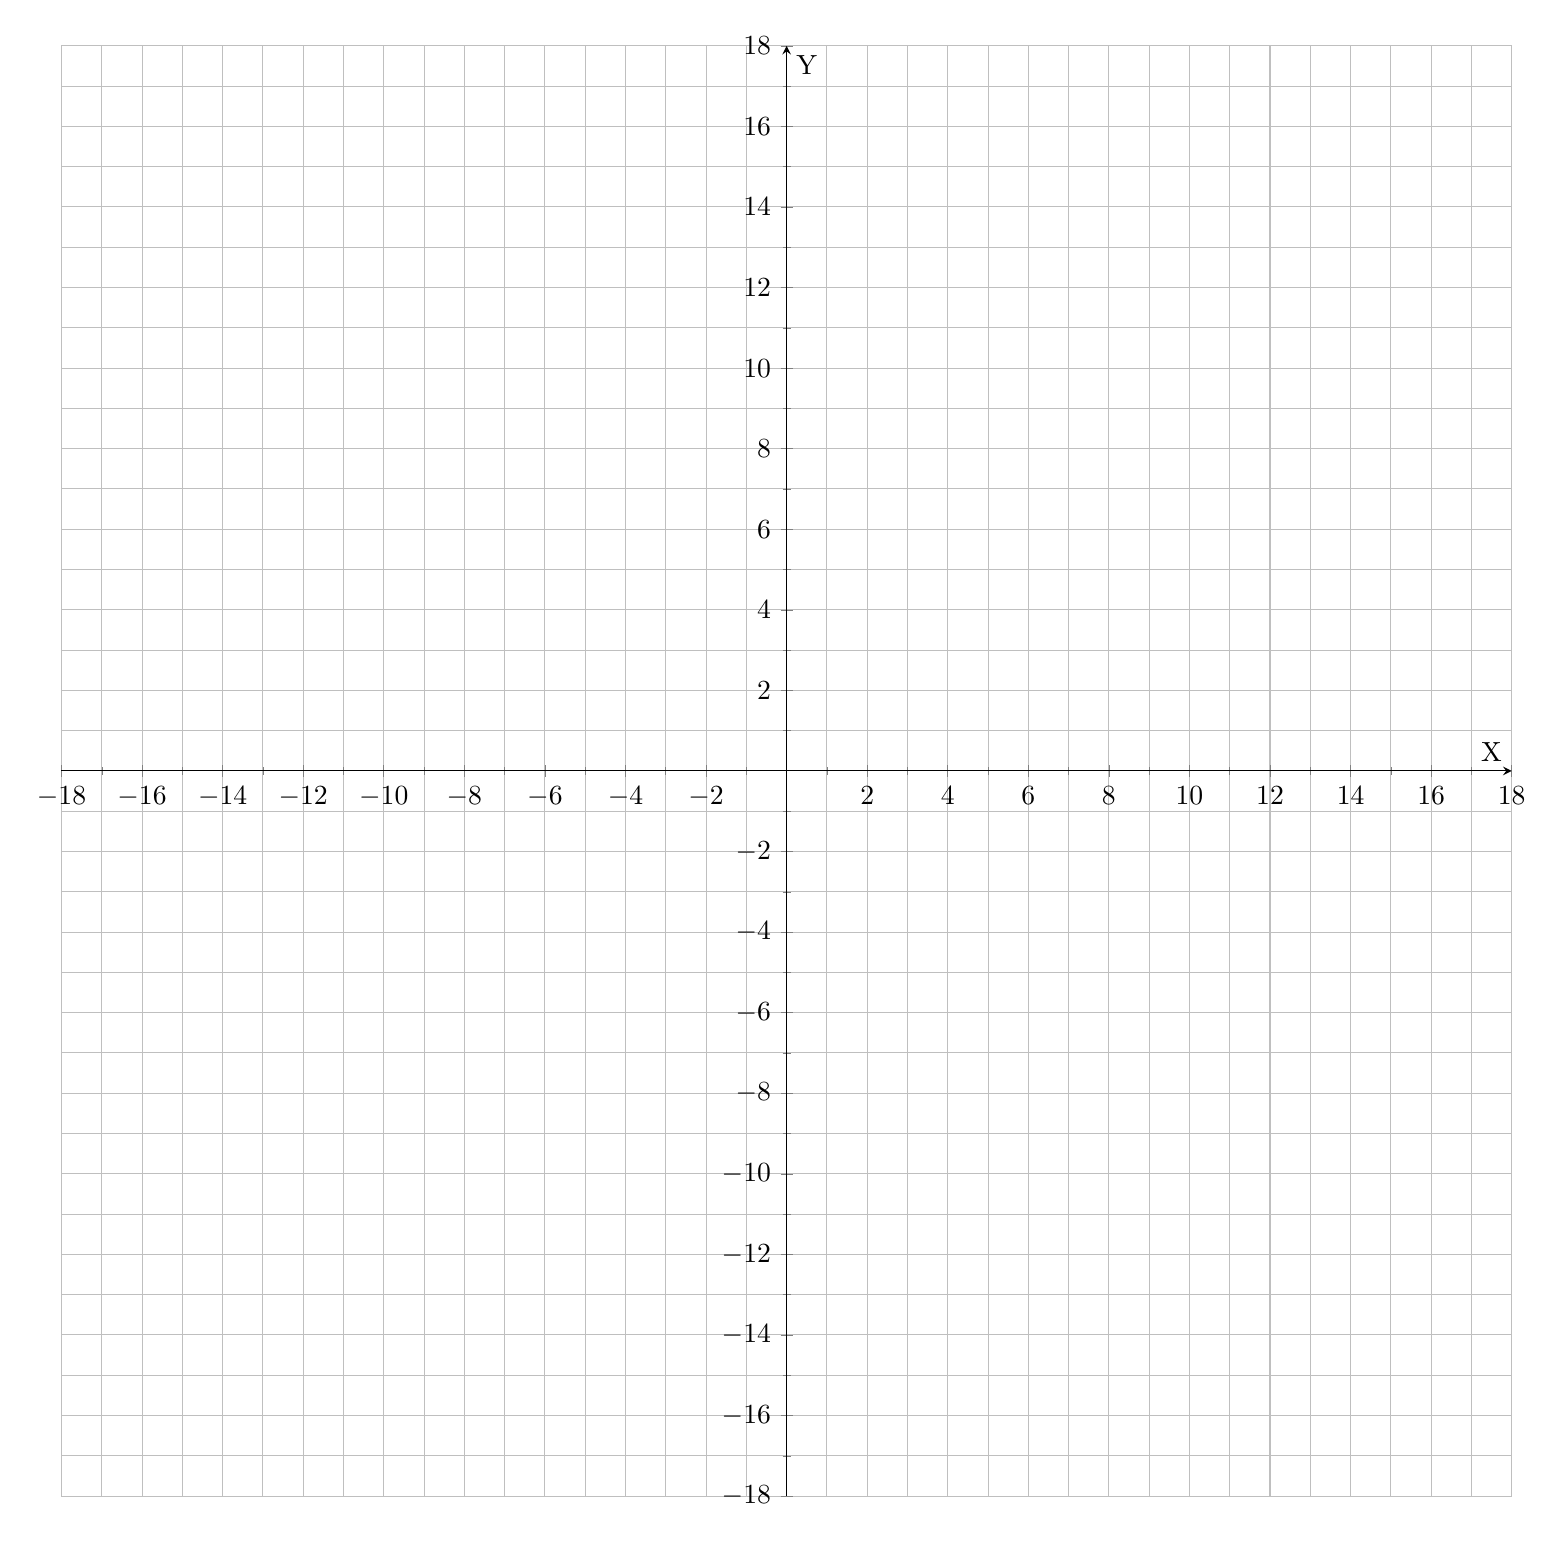
\begin{tikzpicture}
    \begin{axis}[
        axis lines = middle,  % Draw axis lines in the middle
        xmin=-15, xmax=15,  % X-axis range
        ymin=-15, ymax=15,  % Y-axis range
        xlabel={X},  % Label for the X-axis
        ylabel={Y},  % Label for the Y-axis
        grid = both,  % Add grid lines
        minor tick num=1,  % Number of minor ticks
        enlargelimits,  % Enlarge the limits to avoid clipping
        width=20cm,  % Width of the plot
        height=20cm  % Height of the plot
    ]
    \end{axis}
    \end{tikzpicture}

\end{document}
